\documentclass[12pt, a4paper, twoside]{article}
\usepackage[utf8]{inputenc}
\usepackage[spanish]{babel}
\usepackage{hyperref}
\usepackage{fancyhdr}
\usepackage{graphicx}
\usepackage{enumitem}

\pagestyle{fancy}
\fancyhf{}
\fancyfoot[R]{\thepage}
\fancyfoot[L]{\nouppercase{\leftmark}}
\fancyhead[R]{Resumen C\&C en IS.}
\fancyhead[L]{Carlos G. Pérez Aranda. }

\graphicspath{{./Images/}}
\title{Resumen de la asignatura Cognición y Comunicación en Ingeniería del Software}

\begin{document}
\maketitle

\section{hasta el 04/03/2025}

\section{Clase del 04 de marzo.}
Tenemos 4 exposiciones según la imagen adjunta:
\begin{figure}[h]
    \centering
    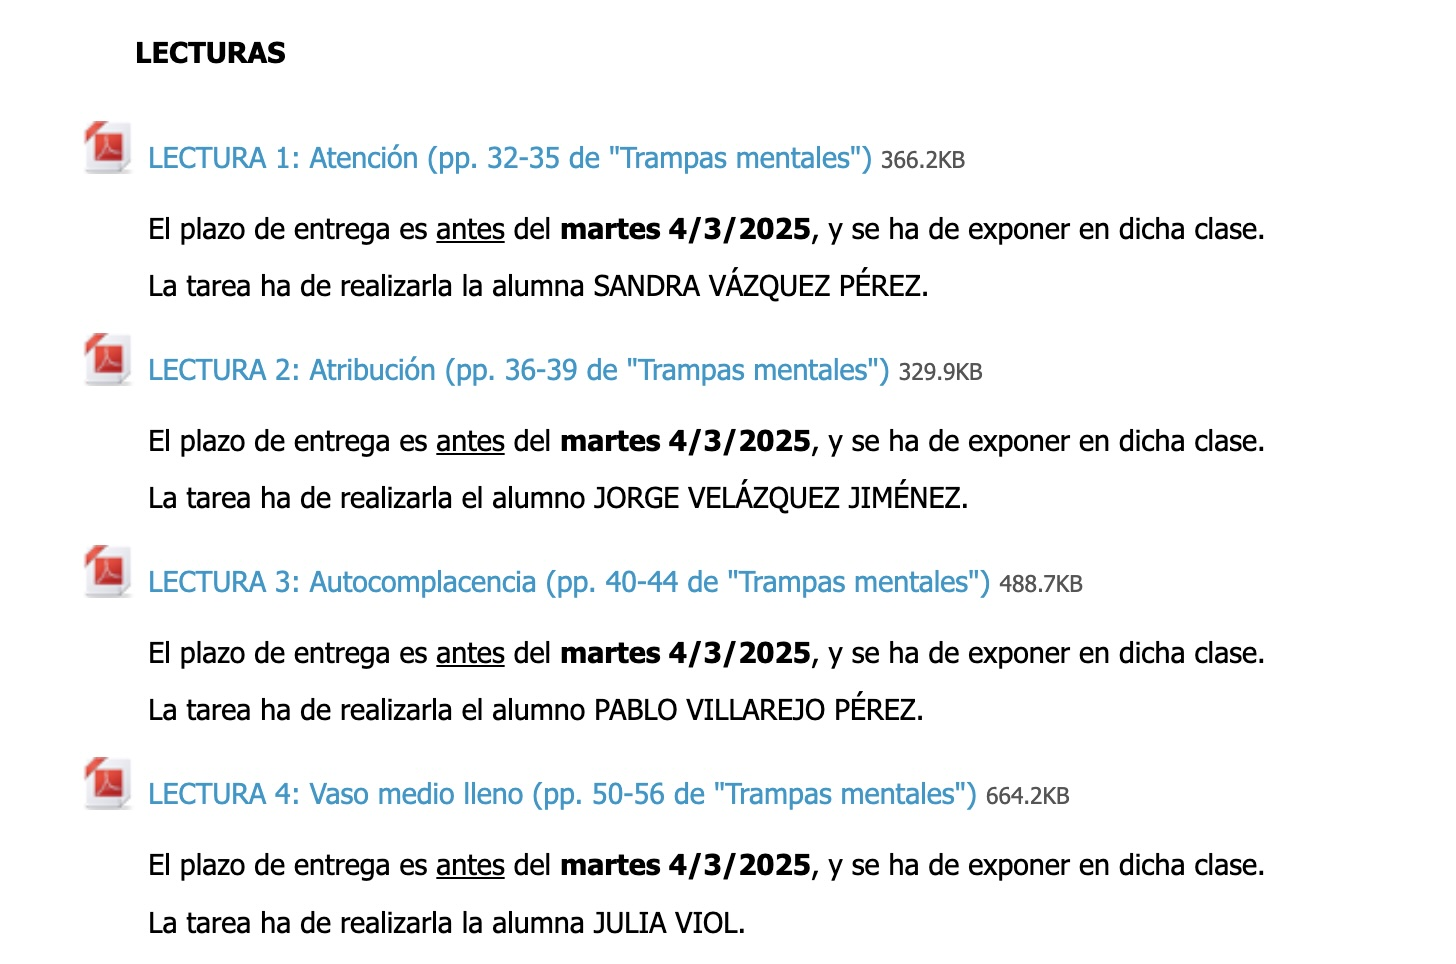
\includegraphics[width=0.9\textwidth]{./Images/0304.jpg}
    \caption{lecturas del día}
\end{figure}

\subsection{Exposición 1 - Trampas mentales}
Como nuestra mente nos engaña. \newline

\subsection{Exposición 1 - Trampas mentales}
Como nuestra mente nos engaña. \\
\begin{itemize}
    \item{Efecto de la ilusión óptica.}
    \item{Efecto de la ilusión de la memoria.}
    \item{Efecto de la ilusión del tiempo.}
    \item{Efecto de la ilusión del espacio.}
    \item{Efecto de la ilusión del control.}
    \item{Efecto de la ilusión de la atención.}
    \item{Efecto de la ilusión del juicio.}
\item {...otros}
\end{itemize}



\subsection{Exposición 2 - Como nos vemos a nosotros mismos en comparación a los demás}
Historia del águila criada con pollos
\begin{itemize}
    \item{Atribución Disposicional: Explicamos el comportamiento de los demás basándonos en su personalidad}
    \item {Atribución Situacional: Explicamos nuestro comportamiento basándonos en la situación}
\end{itemize}
Jones  y Nisbett identificaron que juzamos de manera diferente si somos actores o espectadores..

\begin{itemize}
    \item{Error en el código como falta de habilidad}
    \item{No siempre se considera la presión de los factores externos}
    \item {Puede conllevar baja moral en el equipo.}
\end{itemize}

Kepler estimó 13 días para calcular la órbita de Marte, pero le llevó años.\newline

Fomentar factres situacionales, mejorar la comunicación para evitar atribuciones injustas,
fomentar la empatía y la comprensión.\\

\subsection{Exposición 3 - Autocomplacencia}

La satisfacción por los propios actos o por la propia condición o manera de ser.\newline
Conversación entre Aristipo y Platón.\newline
Somos muy sensibles a los vicios de los demás y ciegos a los propios como mecanismo
de defensa del ego. \newline
\begin{itemize}
    \item{En los éxitos: Soy el mejor.}
    \item{En los fracasos: No es mi culpa, tuve mala suerte.}
\end{itemize}
%% poner en negrita
\textbf{Experimento sobre ansiedad y autocomplacencia:} 

\begin{itemize}
    \item{Bug → La culpa es del lenguaje.}
    \item{Tiempo → El cliente cambió los requisitos.}
    \item{Equipo → No entienden mi código.}
\end{itemize}

\noindent\textbf{Solución:}

\begin{itemize}
    \item{Feedback honesto.}
    \item{Métricas objetivas.}
    \item{Análisis post morten.}
    \item{Primer paso para la mejora es aceptarlo.}
\end{itemize}

\subsection{Lectura 4 - Vaso medio lleno}
Poco que señalar aquí, la presentación fue en inglés, pero aunque entiendo el idioma la 
compañera habló muy bajito y no se escuchaba nada.\\

\subsection{Resumen}
\begin{itemize}
    \item El fondo negro no es adecuado para los proyectores y clases.
    \item Hay que presentarse. Soy fulano de tal y os voy a hablar de ...
    \item El tamaño de letra en el límite.
    \item Hay que moverse por el atril.
    \item Si se hace mención a un vídeo es una oportunidad magnífica para ponerlo.
    \item Poner imágenes en las presentaciones.
    \item Lenguaje no verbal, las manos no en los bolsillos ni cruzados de brazos.
    \item El puntero es un buen apoyo.
    
\end{itemize}

\newpage

\section{Clase del 05 de marzo}

Tenemos 4 exposiciones más según la imagen adjunta:
\begin{figure}[h]
    \centering
    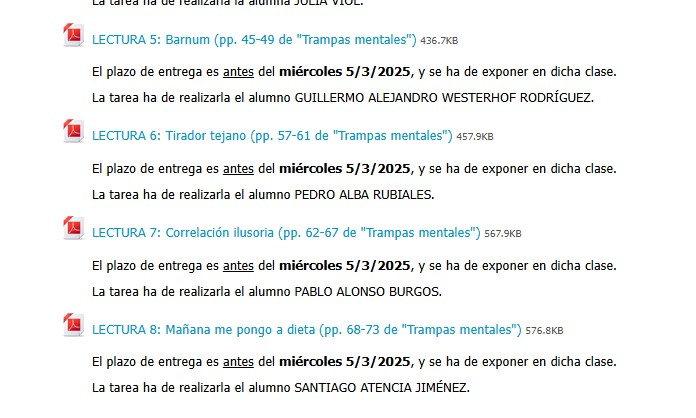
\includegraphics[width=0.9\textwidth]{./Images/0305.jpg}
    \caption{lecturas del día}
\end{figure}

\subsection{Barnum}
Descripción del efecto Barnum y cómo las declaraciones generales pueden parecer personales y precisas.

Falacia de la validación personal.

\subsection{Wishful thinking}
Considerar que algo es más probable o cierto porque se desea que así sea. Este sesgo puede llevar a la toma de decisiones irracionales y a la sobreestimación de las probabilidades de éxito.

\begin{itemize}
    \item{Ejemplo en ingeniería del software: Creer que un proyecto se completará a tiempo a pesar de las señales de advertencia.}
    \item{Solución: Realizar evaluaciones objetivas y basadas en datos.}
\end{itemize}

L'oreal, porque tú lo vales.\newline

Test de personalidad ``Brain works''. El efecto Forer y cómo las personas pueden identificarse con descripciones generales, es más pronunciado en 
personas con trastornos psicóticos, en especial la desorganización cognitiva.

\textbf{Myers-Briggs Type Indicator}, test de personalidad basado en la teoría de Jung. muy usado para
reclutamiento de software y tests de personalidad.\newline

\subsection{Tirador Lejano}
Explicación del sesgo del tirador lejano y cómo se pueden encontrar patrones significativos en datos aleatorios.
\begin{itemize}
    \item Experimento de la moneda. Tirar 4 veces la moneda de 4 en 4 
    \item Exámenes tipo test. Cómo va a salir dos veces seguidas la respuesta b, mucho menos 3 veces.
    \item Incidencia del cancer infantil en una zona por encima de lo normal. Se echa la culpa a factores ambientales.
\end{itemize}

El Tirador Tejano.\newline

Realiza un tiro y luego pinta el blanco. Dando a entender que es un tirador infalible.

\begin{itemize}
    \item Métricas engañosas
    \item Sesgo en validación de datos
    \item Ajuste de requisitos.
    \item Gestión de proyectos, informes de progreso en áreas cn problemas críticos.
    \item Machiune learning. Entrenar un modelo con unos datos que luego se usen para ver la correlación de las predicciones.
\end{itemize}

Solución:

\begin{itemize}
    \item Definir métricas relevantes.
    \item Pruebas rigurosas.
    \item Evitar la manipulación de los requisitos
    \item Revisión de los datos.
    \item Validación cruzada.
\end{itemize}

Tomar decisiones basadas en evidencia real, tener en cuenta la objetividad y el engaño puede llevar a decisiones equivocadas costosas.

\subsection{Correlación ilusoria}
Discusión sobre la correlación ilusoria y cómo las personas pueden percibir relaciones entre eventos que no existen.

Zanahoria y la vista. Es totalmente falsa la correlación entre comer zanahorias y tener buena vista. Lo mismo pasa con los 
amuletos, relacionamos dos hechos independientes.

Debe evitarse decir algo como espero que lo hayan entendido, porque puede llevar a que los oyentes sientan que se les está llamando tontos.


\subsection{Mañana me pongo a dieta}
Reflexión sobre la procrastinación y la tendencia a posponer tareas importantes.

¿Por qué no cumplimos los propósitos de año nuevo?

Pagar para no ir al gimnasio. Mañana será más fácil. Beneficio futuro. 
Coste inmediato para un beneficio futuro.

Cuando queremos hacer algo para el futuro solemos postergarlo. La falacia de la planificación. 
Cuanto tiempo estima un alumno que va a tardar en hacer una tesis, 33.9 días de media. solamente el 30\%
de los alumnos lo terminan en ese tiempo.

Ley Hofstader: Todo lleva más tiempo del que crees, incluso si tienes en cuenta la Ley de Hofstader.

Personas retardatorias, siempre dejan todo para el último momento.

Genera tanto estrés iniciar una tarea que les cuesta mucho empezarla.

\subsection{Conclusiones}

No decir `Me ha tocado tal\ldots'.


No decir `Espero que lo hayan entendido'

Poner transparencia final.

Está bien ponerse como ejemplo de algo, da cercanía.

Poner conclusiones.

\newpage

\section{Clase del 10 de marzo}

Tenemos 4 exposiciones según la imagen adjunta:

\begin{figure}[h]
    \centering
    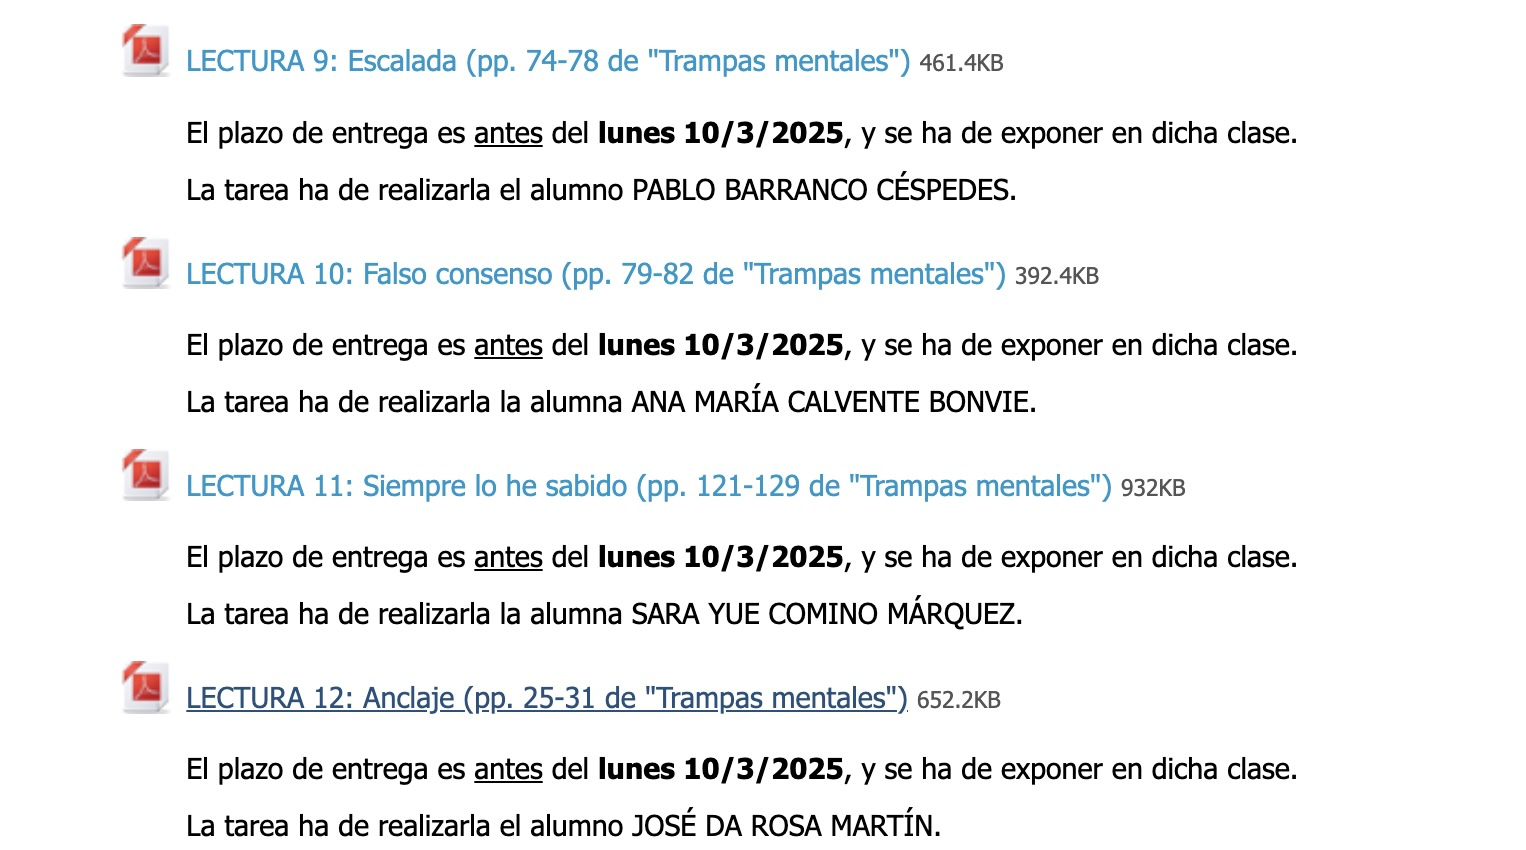
\includegraphics[width=0.9\textwidth]{./Images/0310.jpg}
    \caption{lecturas del día}
\end{figure}

\subsection{Escalada}

Descripción de la escalada de compromiso y cómo las personas pueden continuar invirtiendo en una decisión a pesar de que los resultados sean negativos.

¿Gastaríamos el dinero más a gusto si pudiéramos elegir dónde estamos?

Pone el ejemplo de jugar en un campo de fútbol. Ya que hemos pagado nos quedamos con nuestra elección
aunque no sea la mejor.

Lubik - Experimento de la subasta. Se subasta un billete de 20 euros. La persona que gana la subasta
paga 20 euros y se lleva el billete. La persona que pierde la subasta paga lo que ha pujado y no se lleva nada.

Los que caen en este tipo de juegos son débiles a este efecto.

El Proyecto concorde se pone de ejemplo de este efecto ya que se invirtieron muchos millones en él durante
toda su vida útil.  


Soluciones:

\begin{itemize}
    \item No entrar al juego.
    \item Si entras, tener un plan de salida y ejecutarlo lo antes posible.

\end{itemize}

\newpage
En Desarrollo de Software:
\begin{itemize}
    \item No seguir invirtiendo en un proyecto que no tiene futuro.
    \item No seguir invirtiendo en un proyecto que no tiene futuro.
    \item No seguir invirtiendo en un proyecto que no tiene futuro.
    \item Desarrollo de sw vs costes hundidos
    \item Decisiones de mantenimiento vs reescritura de sw.
    \item Metodologías ágiles y gestión del cambio.
    \item Compra de sw y herramientas.
\end{itemize}


\subsection{Falso Consenso}

Discusión sobre el falso consenso y cómo las personas pueden sobreestimar la cantidad de personas que comparten sus opiniones o creencias.
¿Por qué todos se parecen a mi?.

Lee Ross en los 70. La gente tiende a pensar que los demás piensan como ellos.
Experimento del ``Hombre Anuncio'' en el que se pide a los participantes que lleven un cartel de ``No a la violencia'' y se les pregunta si creen que los demás también llevarán el cartel. La mayoría piensa que sí.
Entre los que aceptaron llevar el cartel, la mayoría pensaba que los demás también lo harían.
Entre los que no aceptaron llevar el cartel, la mayoría pensaba que los demás tampoco lo harían.

Si nosotros elegimos algo pensamos que la mayoría de las personas también lo harían.

Richar Thaler al principio del milenio, escribió un artículo en el Journal of Economics Perspectives en el que hablaba de la economía conductual. En él hablaba de la falacia del falso consenso.
En el que se preguntaba si el sujeto tenía móvil y si pensaba que los demás también lo tenían con resultados análogos al experimento anterior.  

Cuando estamos solos nos fiamos mñas de nuestro propio criterio.

Bernard Whitley - experimento con 260 estudiantes femeninas no casadas.



\subsection{Siempre lo he sabido}

Reflexión sobre la profecía autocumplida y cómo las expectativas pueden influir en el comportamiento y los resultados.


Profetas del día después.

Se hizo un estudio a 160 médicos divididos en dos grupos a los que se les presentó un caso, a uno de los grupos se les dio el diagnóstico
y al otro no. El grupo que tenía el diagnóstico previo tuvo la percepción mayoritaria de que ese era el diagnóstico que hubieran dado, el grupo 
al que no se le facilitó el diagnóstico no tuvo esa percepción (sólo el 30\%).
\newline

Aplicaciones en la ingeniería del software:
\begin{itemize}
    \item Post-morten analysis.
    \item Estimación de costes y tiempos.
    \item Toma de decisiones técnicas.
    \item Análisis de bugs y fallos.
    \item Aprendizaje de proyectos fallidos.
\end{itemize}


\subsection{Anclaje}
Explicación del sesgo de anclaje y cómo las personas pueden depender demasiado de la información inicial al tomar decisiones.\\
\textit{Se aplaza para otro día}


\subsection{\textit{Conclusiones}}
\begin{itemize}
    \item En la diapositiva final poner el nombre de la presentación.
    \item Cuidado con el tamaño de letra.
    \item Si se ponen experimentos, poner los años.
    \item Pocas transparencias en Siempre lo he sabido (sólo 12 transparencias, las otras 15 y 18).

\end{itemize}

\section{Clase del 18 de marzo}

Tenemos 4 exposiciones de las lecturas de la siguiente imagen
\begin{figure}[h]
    \centering
    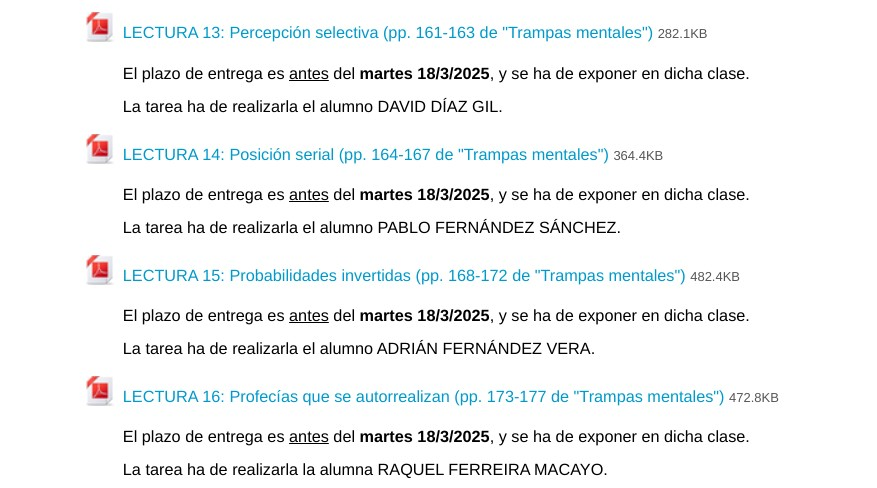
\includegraphics[width=0.9\textwidth]{./Images/0318.jpg}
    \caption{lecturas del día}
\end{figure}
\subsection{Percepción Selectiva}
Validación basada en expectativas.\\
Sesgo en interpretación de bugs.\\
Falsa seguridad en cuanto a la seguridad del software.\\
Programación de errores difíciles de detectar hasta que es demasiado tarde.\\
Daños reputacionales.\\
\subsection{Posición serial}
\subsection{Profecías Autorrealizadas}
Efecto placebo.\\
Definición del efecto placebo.\\
El oráculo de Matrix.\\
\subsection{Conclusiones}


\section{Clase del 19}


\begin{figure}[h]
    \centering
    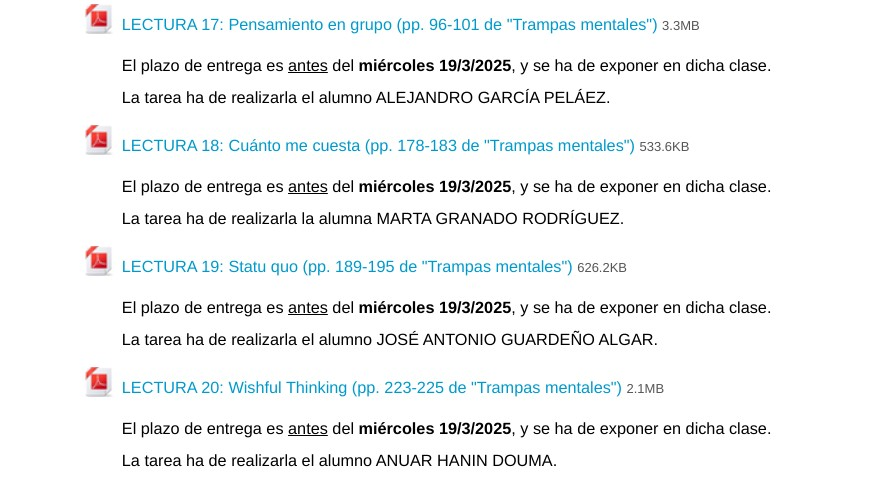
\includegraphics[width=0.9\textwidth]{./Images/0319.jpg}
    \caption{Lecturas del día}
\end{figure}

\subsection{Pensamiento en grupo}
Alumno missing.
\subsection{Cuanto me cuesta}
Tras problemas con el proyector inicia la presentación la compañera.
\subsection{Statu quo}
JA Guardeño.

Resistencia natural al cambio.

El hecho de cambiar la forma de actuar predeterminada cambia la percepción.

\subsection{Conclusiones}
\begin{itemize}
    \item Es bueno grabarse
    \item No cargar de texto las transparencias
    \item Tamaño de letra pequeño no.
    \item Elegir un estilo de diapositiva adecuado a la demanda.
    \item La primera elección condiciona las demás (Status Quo)
    \item Si siempre se tiene razón cómo se va a mejorar.
\end{itemize}


\section{Clase del 25 de marzo}

Tenemos 4 exposiciones de las lecturas de la siguiente imagen
\begin{figure}[h]
    \centering
    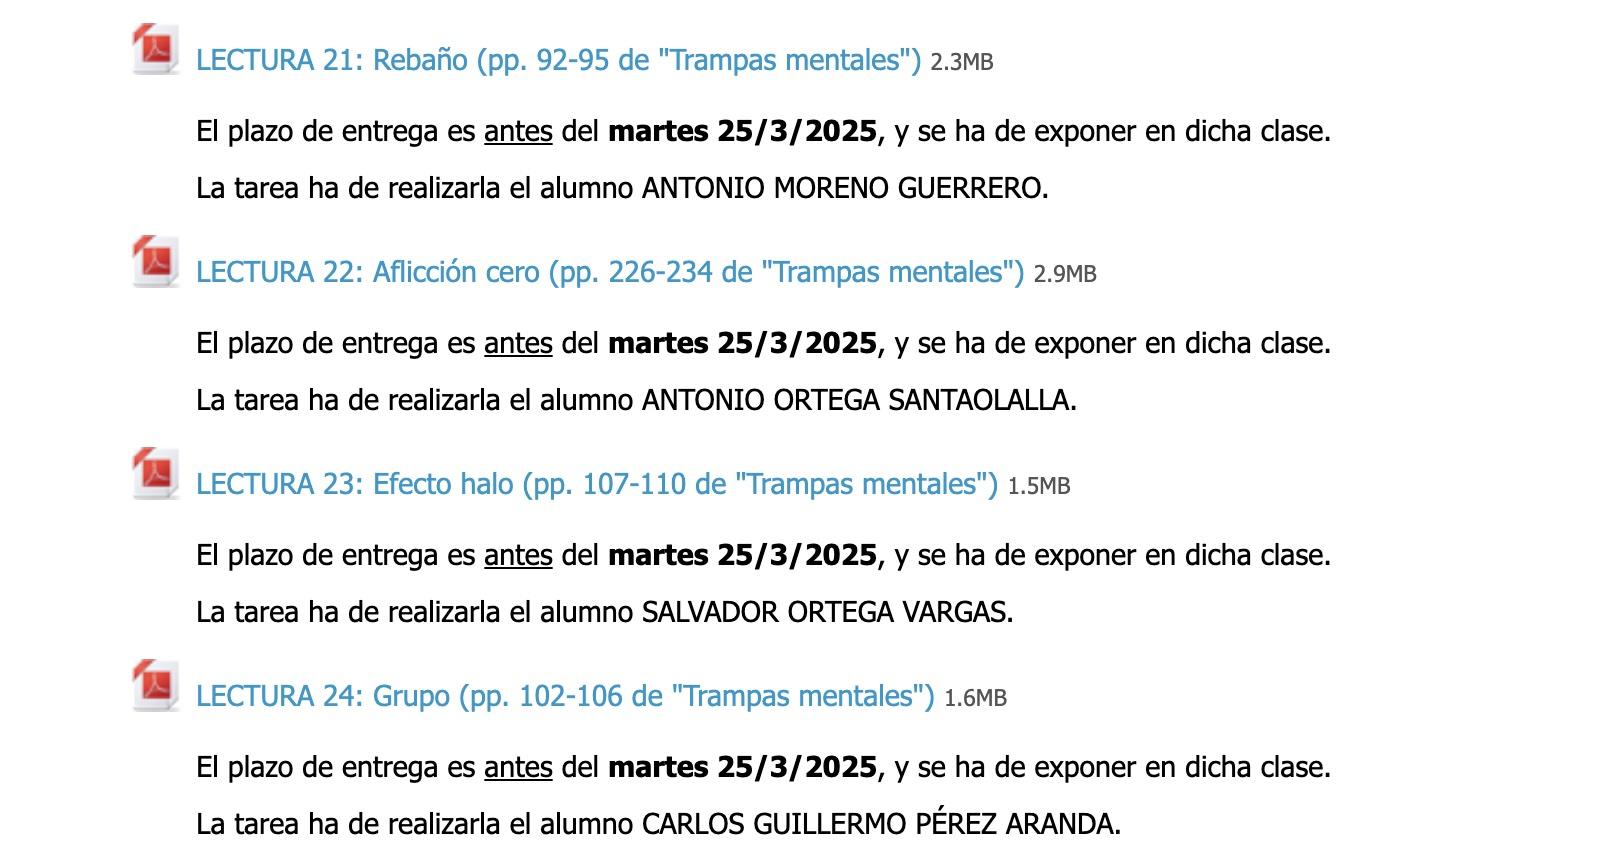
\includegraphics[width=0.9\textwidth]{./Images/0325.jpg}
    \caption{lecturas del día}
\end{figure}

\subsection{Rebaño}

\begin{itemize}
    \item El efecto del rebaño ha creado y destruido imperios.
    \item El efecto del rebaño es la tendencia a seguir a la multitud.
    \item Movilizar a la gente desde el fondo.
    \item Echar la lotería porque la compran los allegados y no voy a ser el único que no la compre.
    \item La gente se fía más de un boca a boca que de un anuncio.
\end{itemize}



\subsection{Aflicción cero}

\begin{itemize}
    \item Duele más perder 100 que satisfacción tenemos en ganar 100.
    \item Sufrimos mas la pérdida que la ganancia.
    \item FOMO Fear Of Missing Opportunity.
    \item Si solo nos lamentamos es una pérdida de energía sin ningún tipo de beneficio.
\end{itemize}

\subsection{Efecto halo}
\begin{itemize}
    \item Ahora hay un halo con la IA.
\end{itemize}

\subsection{Grupo}

Esta es mi exposición.
\subsection{Conclusiones}
\begin{itemize}
    \item En Rebaño: poner alguna trasparencia más de los monos.
    \item Las fechas hay que decirlas, en su defecto los siglos o decenios.
    \item Letra pequeña en el Efecto Halo.
    \item Mirar al público, si hay que concentrarse mirar por encima de las cabezas.
    \item Título de la presentación al final.
\end{itemize}

\section{Clase del 26 de marzo}
    \begin{figure}[h]
        \centering
        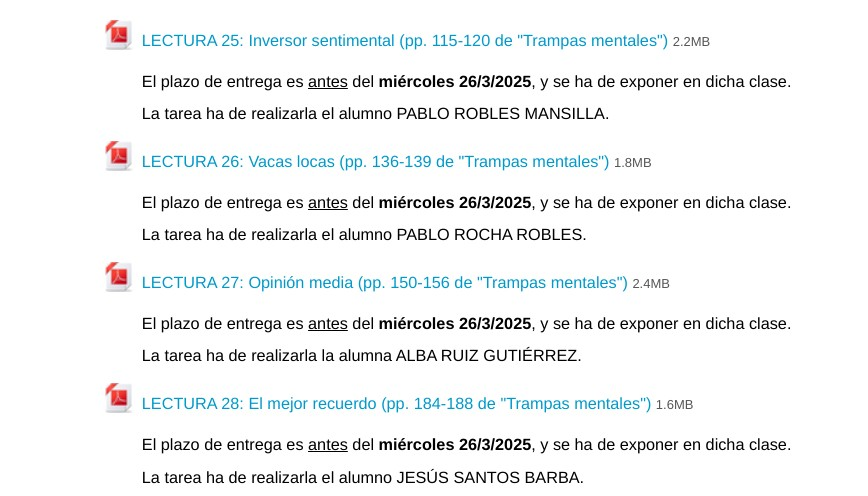
\includegraphics[width=0.9\textwidth]{./Images/0326.jpg}
        \caption{Lecturas del día}
    \end{figure}

    \subsection{Inversor Sentimental}
    El mercado se mueve con las emociones de los inversores.\\
    Zonas cerebrales. Al invertir en una acción se activa la zona del placer del cerebro.
    Cuando se invierte en obligaciones u otros activos seguros y de menor rentabilidad se activa
    la zona del cerebro relacionada con el dolor y las emociones negativas.

    

    \subsection{Vacas Locas}
   
    \subsection{Opinión Media}
    Juego de los 2/3.\\
    La opinión media es la que más se acerca a la realidad.\\
    Me he enterado de poco con la exposición de la compañera.\\
    En general ha tendido a hablar rápido y aunque nos ha invitado a participar casi todos habíamos perdido el hilo.\\
    La teoría del más loco. Last standing loses.\\



    \subsection{El Mejor Recuerdo}
    Recordamos con mayor intensidad del final de una experiencia.\\
    La memoria es selectiva.\\

    \subsection{Conclusiones}
    \begin{itemize}
    \item No meterse las manos en el bolsillo.
    \item Ojo con la letra pequeña.
    \item Si se hace participar al público hay que organizarlo a conciencia para evitar que se pierda la audiencia.
    \end{itemize}

\section{Clase del 31 de marzo} 

Tendremos 1 exposición atrasada y continuaremos con el tema 3.
\begin{figure}[h]
    \centering
    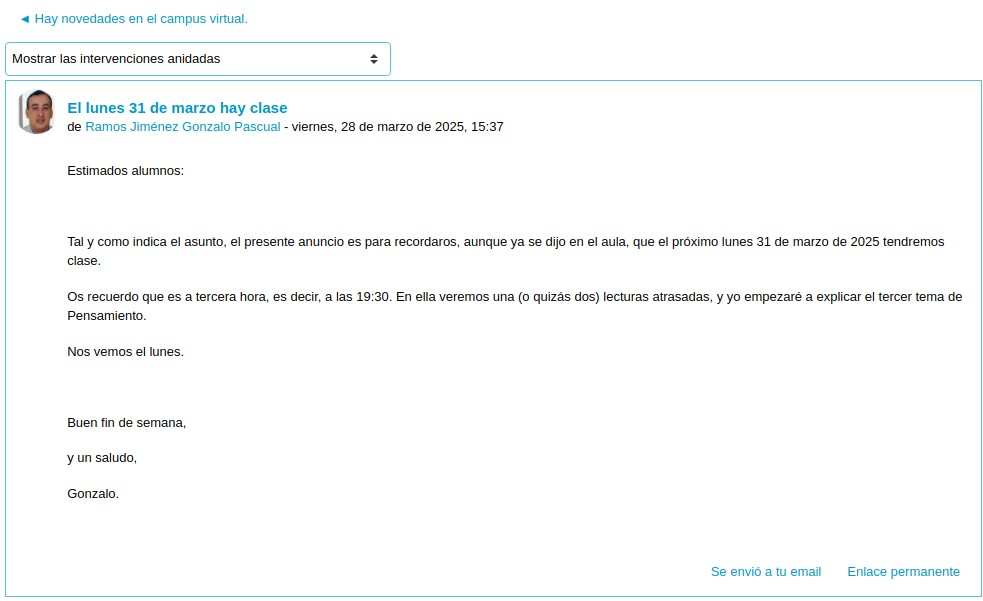
\includegraphics[width=0.9\textwidth]{./Images/0331.jpg}
    \caption{Lecturas del día}
\end{figure}


\section {Tema 3}
Lógica y psicología.\\
\begin{itemize}
    \item{Lógica:} Conexión adecuada entre la premisa y la conclusión.
    
    Todos los mamíferos que conozco con terrestres, luego todos los mamíferos son terrestres.
    La ballena es mamífero, luego la ballena es terrestre.

    Este razonamiento es lógico pero falso.\\

    Si hay un eclipse solar las calles están oscuras.\\
    Hay un eclipse solar, ¿están las calles oscuras?\\
    \item{Validez y veracidad:} Las mujeres embarazadas ganan peso. Mary está ganando
    luego, Mary está embarazada.\\
\end{itemize}
\section{Clase del 1 de abril}
\begin{figure}[h]
    \centering
    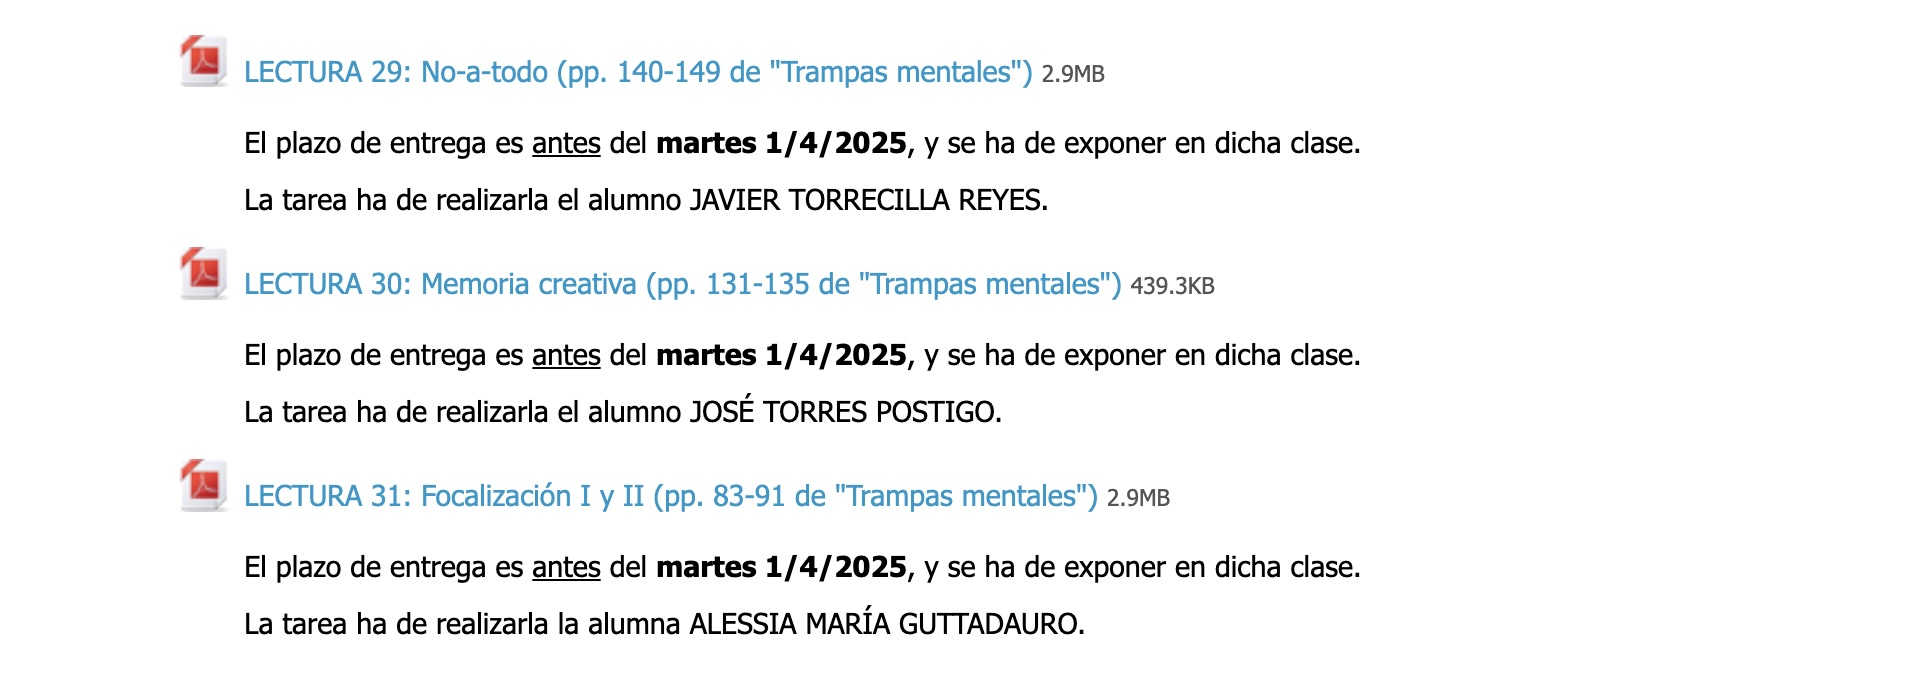
\includegraphics[width=0.9\textwidth]{./Images/0401.jpg}
    \caption{Lecturas del día}
\end{figure}

\subsection{No-a-todo}
La ilusión de la incertidumbre.\\

Evtar riesgos extremos es bueno pero no se pueden eliminar los riesgos totalmente.\\
\subsection{Memoria creativa}
Cuando no recordamos lo que nunca ha sucedido.\\

\subsection{Focalización I y II}
La focalización es la tendencia a centrarse en un aspecto de una situación y no ver el panorama general.\\
Ha sido en italiano, así que me he enterado de poco.\\

\subsection{Conclusiones}
Nuestro cerebro reconstruye la realidad y, a veces, nos engaña.\\
Tomar notas en el momento, en entornos profesionales es fundamental.\\
La memoria se entrena.\\

\section{Clase del 2 de abril}
Comenzamos con las presentaciones de los libros.\\

Hoy presentan los libros:
\begin{itemize}
    \item Sandra Vázquez Pérez: ``Pensamiento crítico. Una actitud''
    \item Pablo Rocha Robles: ``El arte de pensar''
\end{itemize}

\subsection{Pensamiento crítico. Una actitud}
Me gusta que mencione el autor del libro.\\
Se ha confundidido con algunas definiciones.\\
El ejemplo de la libertad en discursos de MartinLuther king y de G. W. Bush 
no está bien hecho, libertad es absoluta y siempre tendrá una connotación positiva.\\
El ejemplo de Alan Sokal tampoco está bien explicado, ¿pasó su artículo la criba por 
que estaba hecho por él, una persona reconocida, o por el contenido del artículo?\\
El de la somalí a la que le retiraron el premio por islamófoba está muy bien explicado.\\

\subsection{El arte de pensar}
Este chaval se traba un poco al hablar.\\
Sócrates el arte de la Mayéutica, se parte de una afirmación que se considera verdadera,
se le da la vuelta y se intenta demostrar que es falsa.\\
El ejemplo ha quedado un poco entrecortado por la expresión del muchacho.\\

\subsection{Conclusiones}
En las conclusiones Gonzalo coincide conmigo.\\

\section{Clase del 8 de abril}
Hoy tenemos las presetaciones de los libros ´´Nuestra Mente Nos Engaña'' a cargo de 
Marta Granado y´´Falacias Lógicas'' a cargo de Pablo Fernández.\\
\subsection{Nuestra Mente Nos Engaña}
Nuestra mente está diseñada para la supervivencia, no para la verdad.\\
Análisis conductual vs cognitivo.\\
Pareidolia. Ver caras en objetos.\\
Error menos letal.\\
Sesgo cognitivo. Cometer siempre el mismo error. Heurística atajo mental para la 
toma de decisiones rápidas. Errores y ruido, variabilidad nconsistente en decisiones
similares.\\
\textbf{Falacia del coste hundido.} Si empiezo algo lo termino.\\
\textbf{Sesgo de grupo.} Como todos lo estamos haciendo tiene que estar bien.\\

Experimento de doble ciego, ni participantes ni investigadores saben si están en el grupo 
de control o en el grupo experimental.\\




Habla un poco rápido, esto hace que no se le entienda bien en ciertas fases de la exposición.\\

\subsection{Falacias Lógicas}

Argumento circular. El testimonio es verdadero porque lo dice el testimonio.\\
Ad Hominem. Atacar a la persona en lugar de al argumento.\\
Ad Populum. Apelar a la mayoría.\\
Pendiente resbaladiza. Si haces esto, luego pasará esto otro.\\
Falsa dicotomía. Si no apoyas esto, apoyas lo contrario.\\




\section{Clase del 22 de abril}
Hoy tenemos las presentaciones de los libros a cargo de Guillermo Alejandro Westerhof
Rodríguez: ``El libro del copywriting'' y David Díaz Gil: ``Tú habla que yo te
leo''

\subsection{El libro del copywriting}

\textbf{Este es un libro que me gustaría leer. Encargado a la biblioteca secreta
y descargado en el kindle.}\\

El copywriting es la técnica de escribir textos persuasivos para vender productos o servicios.\\
Nunca demostrar necesidad en ventas.

Ofrecer gran credibilidad en los argumentos.

Hay que provocar que el cliente te persiga, no tú a él. 
Hay que dar pocos días para que se decida y esperar la confirmación del no interés.

La importancia de decir la verdad y no engañar al cliente. Reconocer errores
fideliza al cliente. Di la verdad incómoda, es más rentable que la mentira 
incómoda.

Las razones auténticas persuaden, las falsas desconfianza.

\subsection{Tú habla que yo te leo}
el 93\% de la comunicación es no verbal.\\
La cara, sonrisa sincera.

Simetría en la elevación de las mejillas.

La duración es natural.\\
Forzada:

Asimetría en la elevación de las mejillas.
No aparecen arrugas alrededor de los ojos.\\


Se puede influuir en nuestro estado de ánimo con la expresión facial.
La expresión facial que forzamos induce al cerebro a pensar que estamos 
sintiendo la emoción que estamos expresando.\\

Bebida caliente predispone a la gente a ser más generosa.\\
Cosas frías predispone para lo contrario.\\

La mirada:
Como identificar al líder de un grupo.

No tiene que ser la persona qué más hable, sino la que recibe más miradas.

Es útil en reuniones en las que hay que identificar a la persona de más poder.\\

La primera impresión.

Los primeros 10 segundos son determinantes, tiende a perdurar y es difícil cambiarla, 
no se ve qué eres.

Nunca hay una segunda oportunidad para una buena primera impresión.\\

Los colores como detonantes de emociones.
El rojo es el color de la pasión, el amor y la energía.\\
El azul es el color de la confianza, la seguridad y la tranquilidad.\\
El verde es el color de la naturaleza, la salud y la frescura.\\
El amarillo es el color de la alegría, la felicidad y la creatividad.\\
Crucial en ámbitos comerciales, color en los logotipos.\\

Te sientes como te vistes.
Nuestra apariencia puede influir en nuestra seguridad y autoestima.\\

La voz. No es lo que decimos sino cómo lo decimos. Tono de voz, volumen, 
silencios, ritmo. Todo lo que pasa por nuestra cabeza se refleja
en nuestra voz.\\

\subsection{Conclusiones}

En mi opinión, las dos exposiciones han sido demasiado largas y monótonas.
No han fomentado la atención y es una pena porque los temas con interesantes.



\section{clase del 23 de abril}

Hoy tenemos las presentaciones de los libros a cargo de Pablo Robles Mansilla: ``Reinventar las organizaciones - Guía ilustrada'' junto con ``Reinventar las
organizaciones'' y Salvador Ortega Vargas: ``Las claves de la creatividad
empresarial''.

\subsection{Reinventar las organizaciones \- Guía ilustrada}
El libro de Frederic Laloux.\\

No me ha despertado interés. 
\subsection{Las claves de la creatividad empresarial}
El libro de José Antonio Marina.\\
Adaptación a cambios por la innovación.

Muchas empresas perciben la innovación como un gasto y no como una inversión.\\
Pensamiento creativo como fuente de innovación.\\
Deducción e inducción. La creatividad está relacionada con la inducción.

Caracteristicas de las personas creativas:
\begin{itemize}
    \item Personalidad.
    \item Autoconfianza.
    \item Percibir los cambios como oportunidades.
\end{itemize}
inteligencia analítica, sintética y la capacidad de persuasión de un individuo.\\

Brainstorming.

\begin{itemize}
    \item No juzgar.
    \item No criticar.
    \item No hacer preguntas.
    \item No hacer comentarios.
\end{itemize}
libertadf, tiempo para innovar, retos estimulantes, evitar la cultura del miedo y 
el conflicto.\\

Estrategia y adaptabilidad $\rightarrow$ Líder alineado con los objetivos de innovación.

Fomentar autonomía y evitar los rankings de los empleados.\\

Dudar $\rightarrow$ Analizar $\rightarrow$ Generar ideas $\rightarrow$ Evaluar $\rightarrow$ Seleccionar $\rightarrow$ Implementar.\\

\section{Clase del 6 de mayo}

Hoy tenemos las presentaciones de los libros a cargo de Javier Torrecilla Reyes:``El poder de un equipo positivo''
y  Pablo Alonso Burgos:``La magia de los equipos extraordinario''.

\subsection{La magia de los equipos extraordinarios}
Me gustaría leerlo.\\
El libro de Patrick Lencioni.\\
Buscar equilibrios entre conservar y cambiar, competir y colaborar, guardar los secretos y compartirlos cn los demás.\\ 

Don Quijote. Viven para trabajar.

Especialista. Trabajador reconocido pero mal gestor.

Enrollado. Se lleva demasiado bien con los empleados, puede hacer que los empleados no le vean como un líder.

\subsection{El poder de un equipo positivo}
Actitud positiva superan desafíos con más facilidad. Mentalidad positiva para que haya reendimiento en el equipo.

Unidad de propósito. Todo el mundo trabaja por un objetivo común.

Resiliencia, capacidad de adaptarse a situaciones adversas.

Cultura positiva, qué tiene el equipo para ser equipo. Tener cultura de base positiva.

Comunicación abierta y honesta. Compartir ideas y hablar críticamente de manera honesta y sincera.

Reconocimiento. Celebrar logros motiva y refuerza comportamientos positivos.

Un equipo se preocupa por el bienestar de todos sus componentes.


\section{Clase del 7 de mayo}
Hoy tenemos las presentaciones de los libros a cargo de Santiago Atencia Jiménez: ``Negociar lo imposible''
y  Anuar Hanin Douma: ``Negociar es fácil, si se sabe cómo''

\subsection{Negociar lo imposible}
El libro de William Ury.\\

Ejemplo de la negociación de los ingresos de la NFL.

Saber manejar el procedimiento de la negociación te da poder a la hora de negociar.

Negociaciones de guerra Vietnam, tratado de París.
Empatía, La Crisis de los Misiles de Cuba.
Negociar con una pistola en la cabeza. 


\subsection{Negociar es fácil, si se sabe cómo}
El libro de José Antonio Marina.\\

Negociación con clientes y stakeholders.\\

Gestión de equipos con escucha activa.

Negociación en Metodologías ágiles.

Acuerdos con proveedores.

Negociar no es imponer sino colaborar con inteligencia.

\subsection{Conclusiones}

Negociar es importantísimo. Hay que saber negociar.
Estamos todo el día negociando, sobretodo en el ámbito laboral.

El poder de la formulación. Cómo presento las cosas.

\section{clase del 12 de mayo}
Tras el kahoot que quedaba empezamos con el tema 4.
Heurísticos y sesgos.

\begin{itemize}
    \item{Heurístico de disponibilidad:} Tendencia a juzgar la probabilidad de un evento basándose en ejemplos recientes o memorables.
    \item{Heurístico de representatividad:} Tendencia a clasificar algo en función de su similitud con un prototipo.
    \item{Heurístico de anclaje:} Tendencia a depender demasiado de la primera información recibida al tomar decisiones.
    \item{Heurístico de afecto:} Tendencia a tomar decisiones basadas en emociones y sentimientos.
\end{itemize}

Limitaciones de nuestro sistema cognitivo.\\
\begin{itemize}
    \item Temporales: tiempo escaso.
    \item Datos: Información limitada o incompleta.
\end{itemize}




\end{document}